\section{Experimental Set-up\label{sec:VT-experimentalSetUp}}
\subsection{Optical Trap\label{sec:VT-opticalTrap}}

The optical trap is based on the apparatus described in detail elsewhere 
\cite{Bodensiek}. We modified and enhanced the standard setup and its 
peripherals such that it is suitable for our micro-fluidic applications. These 
applications require a long term laser stability, fine spatial resolution in 
three dimensions, spatial reproducibility of the positioning system, and fine 
temporal resolution of the DAQ system. The taken measures are explained in the 
following.

The collimated beam of a \SI{200}{\milli\watt} (lineary polarized in the 
$yz$-plane, $<$0.5\% power drift in \SI{8}{\hour}), \SI{785}{\nano\meter} near 
infrared laser diode (LuxX 785-200, Omicron Laserprodukte GmbH, 
Rodgau-Dudenhofen, Germany) is coupled into a standard microscope chassis (Nikon 
NI-U, Tokyo, Japan).  Although the laser is linearly polarized, it forms a 
symmetric optical trapping potential by focusing the laser beam with a water 
immersion microscope objective (CFI Plan Apo IR SR 60XWI 1.27NA, Nikon, Japan) 
with a high numerical aperture (NA) of 1.27. Immersol W with a refractive index 
of $n=1.33$ at room temperature (Zeiss, Germany) is used as an immersion media 
instead of water to obtain a higher temporal stability of acoustic standing wave 
modes during the experiments \cite{Lamprecht2016}.  Downstream of the focused 
laser beam, the laser light is collimated again by an air condenser (C-C Abbe NA 
0.9, Nikon, Japan) and split into two separate beams by a non-polarizing 50:50 
beam splitter (CCM1, Thorlabs, USA). A schematic sketch of the optical set-up 
and the focused laser inside an acoustofluidic flow cell is shown in 
\cref{fig:Fig2}.

%%%%%%%%%%%%%%%%%%%
\begin{figure}[tb]
    \centering
    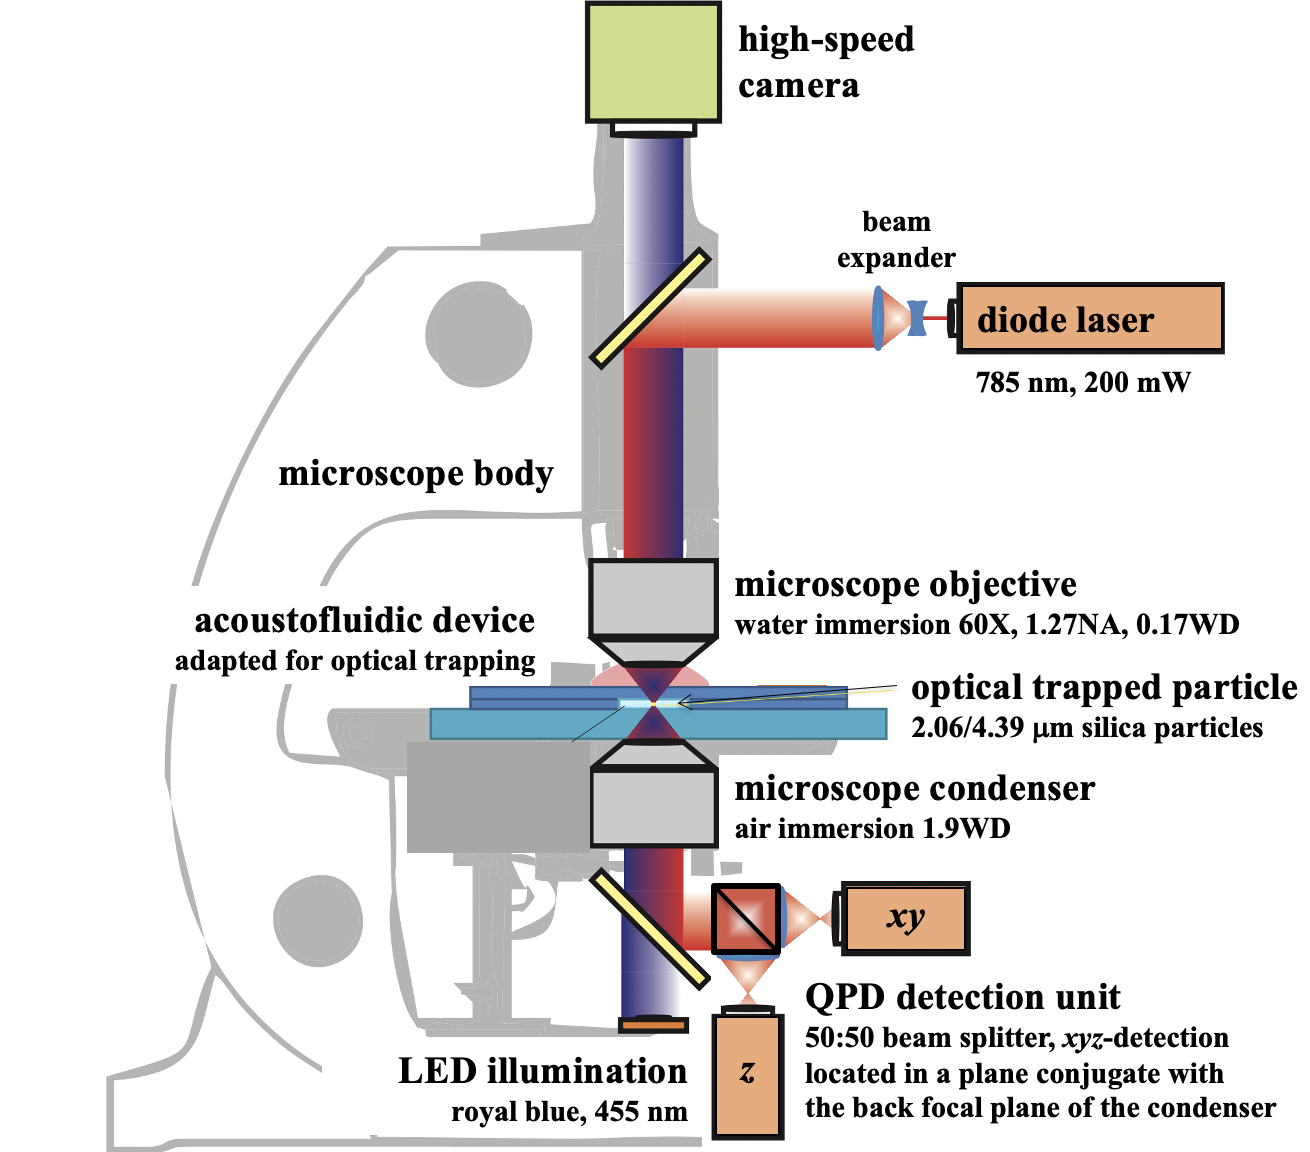
\includegraphics[width=84mm]{Fig2.png}
    \caption{The optical trap is based on a commercial upright microscope body.  
        The linear polarized laser light (\SI{785}{\nano\meter}) is aligned on 
        an optical table and coupled into the microscope. The microscope 
        objective forms the laser focus for trapping, and the condenser directs 
    the laser light to the detection unit, where QPDs are used for the analysis 
  of the particle displacements. An LED illuminates the sample and a high-speed 
camera is used for imaging.\label{fig:Fig2}}
\end{figure}%
%%%%%%%%%%%%%%%%%%%

The laser beam is projected onto a Quadrant Photo Detector (QPD) that is 
conjugated with the back focal plane of the condenser \cite{Bodensiek}. The 
QPD-$xy$ in \cref{fig:Fig2} is optimized to detect the $xy$-displacement of 
optically trapped particles. The laser spot size on the QPD-$xy$ is about 
\SI{2}{\mm} in diameter and the \SI{8}{\mm} diameter sensor measures 
displacements of the beam in the back focal plane. The QPD-$z$ measures the 
total laser intensity over its four quadrants which scales with the 
z-displacement of the particle inside its optical potential \cite{Dreyer}.

The analog data of the QPDs is anti-aliasing filtered at \SI{15}{\kilo\hertz} 
and is digitized by a data acquisition board (NI USB-6356, National Instruments, 
Austin, TX, US) with a sampling frequency of \SI{1}{\MS} (1 million samples per 
second). We recorded the Brownian motion of the particle within the optical trap 
for ten seconds and then performed a Fast Fourier Transform (FFT) on this signal 
to achieve a frequency resolution of $\Delta f=\SI{0.1}{\hertz}$. This spectrum 
is averaged over 10 cycles such that the calibration takes \SI{100}{\second}.  
The recorded signals are then further processed for calibration and force 
measurements in 3D with a self-written Matlab and LabVIEW (National Instruments, 
Austin, TX, US) routine.  Calibration of the position (\si{\meter\per\volt}) and 
force sensitivity (\si{\newton\per\meter}) was obtained via the Equipartition 
Theorem \cite{Svoboda,Vermeulen}. These calibrations are performed for the $x$-, 
$y$- and $z$-directions simultaneously. Due to the elongated shape of the focal 
spot in the $z$-direction, the optical trap stiffness $\kappa_z$ is 3 to 5 times 
weaker than the trapping stiffness in $x$- and $y$-direction. 

Here, a typical optical trapping stiffness for \SI{100}{\milli\watt} laser power 
and \SI{2.06}{\micro\meter} silica particles is 
\SI{2.9}{\femto\newton\per\micro\meter} in the $xy$-plane and 
\SI{1.1}{\femto\newton\per\micro\meter} in the $z$-direction. During the 
experiments it was ensured with the magnitude of the laser power that the 
displacements $u$ of the particles remained inside the valid regime of the trap 
calibration ($u<\sfrac{R}{2}$). The main counteracting force is the acoustic 
radiation force. With our Optical Trap setup we can stably trap particles 
between \SI{2}{\micro\meter} to \SI{10}{\micro\meter}. Larger particles tend to 
show unstable trapping in our setup.
% unstable trapping in our setup; smaller particles get closer to the used laser 
% wavelength ($\lambda = \SI{785}{\nano\meter}$) whereas our calibration method is 
% derived for $\lambda < R_{\text{particle}}$.

The spatial positioning of the optical trap in the $xy$-direction and 
$z$-direction was performed by a closed-loop motorized microscope stage (SCAN, 
Marzhauser, Wetzlar, Germany) and closed-loop piezo stage (PI, P-725.2CD, 
Karlsruhe, Germany), respectively. The statistic force repeatability of the 
optical trapping set-up was $\pm \SI{11}{\femto\newton}$ \cite{Lamprecht2016}, 
which includes positional drifts and eventual variations in temperature.

\subsection{Acoustofluidic Flow Cell\label{sec:VT-DeviceAndAcoustics}}

Within the optical trap, the working distance of the microscope objective 
(\SI{0.17}{\milli\meter}) and of the condenser (\SI{1.9}{\milli\meter}) limits 
the thickness of the flow cell.  Furthermore, the device has to be transparent 
for the laser wavelength $\lambda$ to permit optical trapping and detection (see 
\cref{fig:Fig2}). Therefore, a transparent glass device was built from a stack 
of standardized microscope coverslips (MENZEL GmbH, Braunschweig, Germany). It 
was designed to excite two individual standing waves in $x$- and $y$-direction 
separately, which provide the necessary conditions to rotate spherical 
\si{\micro\meter} particles. 

Similar as in \citeauthor{Lakamper} \cite{Lakamper}, a polyurethane spray glue 
(ITW, Cramolin Urethan, Muehlacker, Germany) was used for the fabrication of the 
micro-fluidic flow cells. Two square shaped coverslips of size (thickness, 
\numrange{0.13}{0.17} \si{\milli\meter}, and \SI{22x22}{\mm} large) were glued 
together and afterwards a \SI{4.0}{\milli\meter} wide cross-shaped fluid channel 
was diced into the center of one of the two coverslips. The remaining material 
of the diced coverslip was covered by another adhesive layer and glued onto a 
rectangular glass (thickness, \numrange{0.13}{0.17} \si{\milli\meter}, 
\SI{60}{\mm} long, \SI{22}{\mm} wide). The resulting stack of coverslips formed 
two crossed fluid channels in $x$- and $y$-direction with open ends (soft 
acoustic boundaries). The maximal distance of the fluid cavity depth plus the 
top cover thickness is $< \SI{270}{\micro\meter}$ as depicted in 
\cref{fig:Fig3}. An adapted phenolic paper with the size of a standard specimen 
slide ($l$, $w$, and $h$ = \numlist{75; 25; 1} \si{\mm}) holds the stacks of 
coverslips, so that the acoustic flow cell can be easily placed in the sample 
holder of the microscope stage.

%%%%%%%%%%%%%%%%%%%
\begin{figure}
    \centering
    \includegraphics[width=84mm]{Fig3.png}
    \caption{Stack of three coverslips form the device where the middle layer 
    includes two fluid channels (\SI{4.0x22}{\mm} with a depth of 
    \numrange{0.13}{0.17} \si{\milli\meter}, red boxes) in an orthogonal 
    arrangement. The two channels intersect and form a \SI{4.0x4.0}{\mm} crossed 
    chamber (black hatched area). Each piezo-electric transducer 
    \SI{4.0x2.0x0.5}{\mm} (PZ26, blue boxes) individually excites a direction.  
    The relative phase difference $\zeta$ of the excitation signals is freely 
    adjustable. The phenolic paper holds the stack and has the size of a 
    standard specimen slide for mounting.\label{fig:Fig3}}
\end{figure}
%%%%%%%%%%%%%%%%%%%

Two piezo-electric transducers (Ferroperm, Pz26, $l$, $w$, and $h$ = \numlist{4; 
2; 1} \si{\mm}, Kvistgaard, Denmark) were glued on the stack of coverslips with 
conductive glue (EPOXY Technology, H20E, Billerica, MA, USA) perpendicular to 
each channel in $x$- and $y$-direction. The distance between the center of the 
fluidic chamber and each transducer was \SI{7}{\mm}. This distance was set such, 
that the microscope objective stays clear from the transducers. The resulting 
thin design of the device ensured the usage of the optical trap and decoupled 
the standing wave modes in the channels ($x$ and $y$). This specific design 
enabled controlled excitation of standing wave modes in the directions of $x$ 
and $y$ as well as an individual control of the excitation phase $\zeta$ (see 
\cref{fig:Fig4}).

For our measurements we always used the same spatial position within the device.  
Hence, the rotation of the particles is always in the same direction for our 
experiments. However, \citeauthor{lamprecht2015} \cite{lamprecht2015} 
demonstrated how the rotation direction is dependent on the spatial location and 
the phase $\zeta$ of the two standing waves. In addition, in the supplemental 
material two videos are provided that show the change of rotation direction when 
changing these two parameters.

%%%%%%%%%%%%%%%%%%%
\begin{figure}
    \centering
    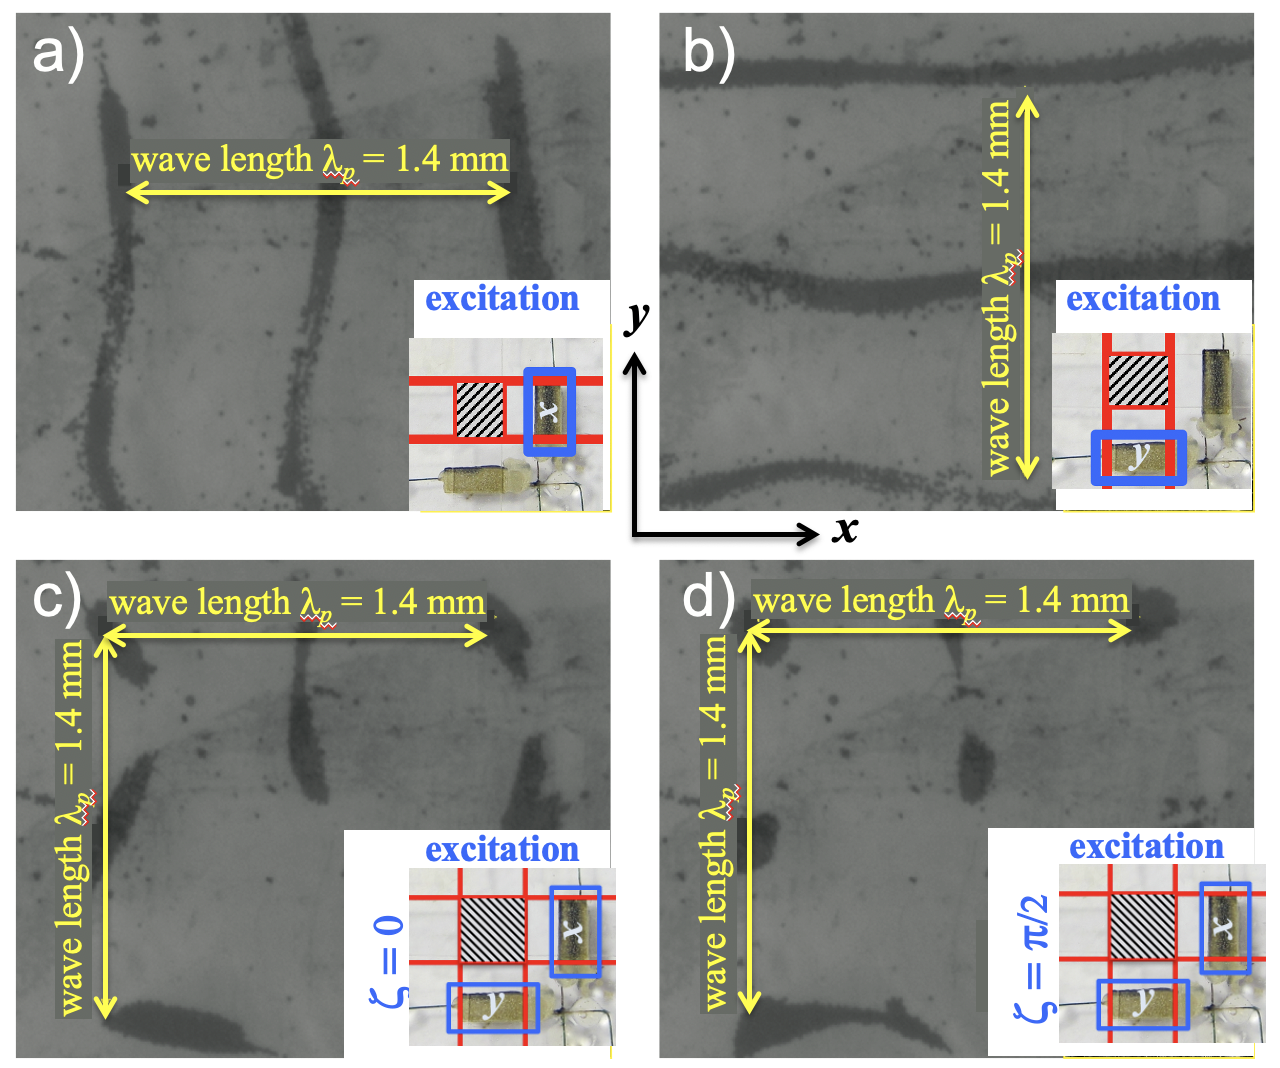
\includegraphics[width=84mm]{Fig4.png}
    \caption{The device is filled with a water/glycerol (70$\%$/30$\%$) mixture 
    containing \SI{4}{\micro\meter} copolymer particles (Duke Scientific 
    Cooperation, Palo Alto, CA, USA) and it has two identical modes in $x$- and 
    $y$-direction at \SI{1.043}{\mega\hertz}. a) and b) depict the isolated 
    modes at \SI{15}{\Vrms} for the $x$- and $y$-direction, respectively. The 
    resulting measured wavelength $\lambda_{P}$ was approximately 
    \SI{1.4}{\milli\meter} for both directions.\ c) and d) show the particle 
    pattern for the two orthogonal standing waves inside the crossed-fluid 
    chamber at $\zeta= 0$ and $\zeta= \frac{\pi}{2}$, respectively. These 
    observations confirm the assumption of a 2 dimensional orthogonal standing 
    wave field.\label{fig:Fig4}}
\end{figure}
%%%%%%%%%%%%%%%%%%%


\subsection{Particles \label{sec:VT-particles}}
For the visualization experiment in \cref{fig:Fig4} we used \SI{4}{\micro\meter} 
copolymer particles (Duke Scientific Cooperation, Palo Alto, CA, USA). For the 
optical trapping experiments with single particles we used silica particles 
because they are more precise in their dimensions compared to polystyrene 
particles. In addition, they have better interactions
with the acoustical field. Moreover, the results of \citeauthor{hahn2016} 
\cite{hahn2016} suggest that in the region of $R \approx \delta$ and ratios of 
$\sfrac{\rho_{\text{s}}}{\rho_{\text{f}}}$ between 2 and 15 result a greater 
magnitude of the acoustic viscous torque results. With the used fluid ($\rho_{f} 
= \SI{1.1}{\gram\per\cubic\centi\meter}$) and our silica particles ($\rho_{s} = 
\SI{2.0}{\gram\per\cubic\centi\meter}$) the ratio 
$\sfrac{\rho_{\text{s}}}{\rho_{\text{f}}} \approx 1.8$.

In order to validate the proposed power spectrum method two sets of validation 
experiments are explained in \cref{sec:VT-rotationDetectionValidation}. For those 
the \SI{4.39}{\micro\meter} particles were modified differently for each 
experiment. We use this size of particles since they are better visible when 
simultaneously measuring the rotation with a camera. There was the need to 
\emph{mark} the spherical \SI{4.39}{\micro\meter} silica particles because a 
reliable rotation measurement with the camera of unmarked spherical particles 
was not possible.

Two methods for marking were used. In both cases the rotation could be easily 
tracked by optical microscopy because the particle size of 
\SI{4.39}{\micro\meter} silica glass micro-spheres (Microparticles
GmbH, Berlin, Germany) is much larger than the optical resolution.
For the set of experiments, silica particles were deformed between two polished 
metal plates by applying a pressure of \SI{1}{\mega\pascal} to achieve a slight 
degree of non-sphericalness (see \cref{fig:Fig5}). For the second set, uncoated 
particles were distributed on a glass specimen slide (MENZEL GmbH, 
Menzel-Glaesser, Braunschweig, Germany) and coated by a Sputter coater (B7340 
Manual Sputter Coater, Van Loenen Instruments, Zaandam, Netherlands) with a gold 
coating (see \cref{fig:Fig6}). After coating, the particles were half-covered 
with a \SIrange{10}{20}{\nano\meter} thick gold layer at their surface 
orientated to the gold electrode. The coating affected the acoustic properties 
not substantially. The particles showed, i.e., same trapping and rotational 
behavior within the acoustical trap. Averted particle surfaces showed a thinner 
gold layer of about \SIrange{0}{10}{\nano\meter}.
